% !TeX spellcheck = fr_FR
\documentclass[a4paper,11pt,oneside,roman]{article}
    \usepackage[utf8]{inputenc}
    \usepackage[T1]{fontenc}
    \usepackage[top=2cm, left=2cm, right=2cm, bottom=2cm]{geometry}
    \usepackage[francais]{babel}
    \usepackage[hidelinks=true]{hyperref}
    \usepackage{listings}
    \usepackage{color}
    \usepackage{amsmath}
    \usepackage{graphicx}
    \usepackage{amssymb}
    \usepackage{natbib}
    \usepackage{float}
    \usepackage{hyperref}
    \usepackage{advdate}
    
    \floatplacement{figure}{H}
    
    \definecolor{dkgreen}{rgb}{0,0.6,0}
    \definecolor{gray}{rgb}{0.5,0.5,0.5}
    \definecolor{mauve}{rgb}{0.58,0,0.82}
    
    \linespread{1.3} %space between lines
    \setlength{\parskip}{1em}  %space between paragraphs
    
    \begin{document}
    
    \begin{titlepage}
    
        \newcommand{\HRule}{\rule{\linewidth}{0.5mm}} % Defines a new command for the horizontal lines, change thickness here
        
        \center % Center everything on the page
         
        %----------------------------------------------------------------------------------------
        %	HEADING SECTIONS
        %----------------------------------------------------------------------------------------
        
        \textsc{\LARGE Université de Technologie de Compiègne}\\[0.5cm] % Name of your university/college
        \textsc{\Large Génie informatique}\\[1.5cm] % Name of your university/college
        
        %----------------------------------------------------------------------------------------
        %	TITLE SECTION
        %----------------------------------------------------------------------------------------
        
        \HRule \\[0.4cm]
        { \huge \bfseries Entrainement d'un réseau de neurones et rétropropagation dans le cadre d'un problème de classification.}\\[0.4cm] % Title of your document
        \HRule \\[1.5cm]
         
        %----------------------------------------------------------------------------------------
        %	AUTHOR SECTION
        %----------------------------------------------------------------------------------------
        
        % If you don't want a supervisor, uncomment the two lines below and remove the section above
        \Large \emph{Authors:}\\
        Nacim \textsc{Khalis} et Antoine \textsc{Collas}\\[3cm] % Your name
        
        %----------------------------------------------------------------------------------------
        %	DATE SECTION
        %----------------------------------------------------------------------------------------
        
        {\large \AdvanceDate[-4]\today}\\[4cm] % Date, change the \today to a set date if you want to be precise
        
        %----------------------------------------------------------------------------------------
        %	LOGO SECTION
        %----------------------------------------------------------------------------------------
        
        
\includegraphics[width=0.5\textwidth]{imgs/logo_UTC_SU.jpg}\\[1cm] % Include a department/university logo - this will require the graphicx package
        
        %----------------------------------------------------------------------------------------
        
        \vfill % Fill the rest of the page with whitespace
        
    \end{titlepage}
    
    % \tableofcontents
    
    \pagebreak
        
    \section{Réseau de neurones: perceptron}
    
    L'objectif est de programmer un perceptron afin de classer un ensemble de bouteilles de vins en 3 ensembles (dataset disponible \href{http://scikit-learn.org/stable/modules/generated/sklearn.datasets.load_wine.html}{ici}). 
    Dans la suite de ce document nous souhaitons entrainer un perceptron ayant une couche cachée sur cet ensemble de données.

    L'architecture de notre perceptron est la suivante:
    \begin{figure}
        \centering
        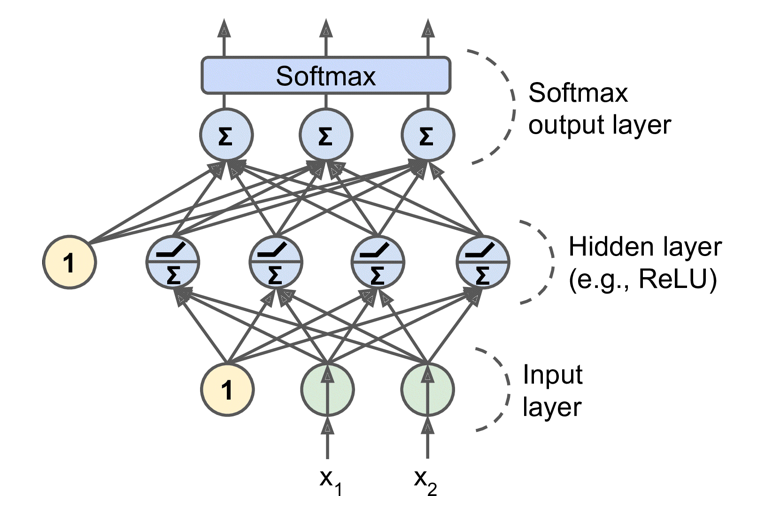
\includegraphics[width=0.5\textwidth]{imgs/perceptron.png}
        \caption{Perceptron multi-couches tiré de \cite{geron}.}
        \label{fig_perceptron}
    \end{figure}

    Le réseau est composé d'une couche d'entrée avec 13 neurones (les bouteilles de vins ont 13 caratéristiques et donc sont représentées par des vecteurs de 13 dimensions), une couche cachée avec un nombre de neurones à régler (un hyperparamètre de notre réseau de neurones) et de 3 sorties (une sortie par classe à prédire).
    La fonction d'activation est une fonction RELU: $RELU(x) = max(0,x)$. 
    
    \begin{figure}
        \centering
        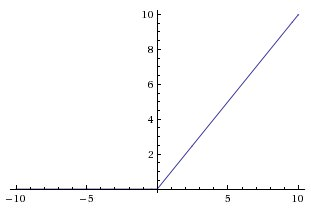
\includegraphics[width=0.5\textwidth]{imgs/RELU.jpg}
        \caption{Fonction RELU.}
        \label{fig_relu}
    \end{figure}
    
    Le choix de cette fonction d'activation est motivé par les raisons suivantes (tirées de \cite{pmlr-v15-glorot11a}):
    \begin{itemize}
        \item Rapide à calculer.
        \item Biomimétisme. Tout d'abord La fréquence d'impulsions d'un neurone biologique en fonction de l'intensité reçue peut être assimilée à une fonction RELU.
        En effet, la fréquence d'impulsions d'un neurone biologique est une fonction de l'intensité reçue en entrée. 
        En dessous d'un certains seuil le neurone biologique ne renvoie aucune impulsion.
        Au dessus de ce seuil la fréquence d'impulsions croit linéairement par rapport à l'intensité reçue (jusqu'à $1\times 10^{-9} A$). Cette linéarité est visible dans le carré rouge de la figure \ref{fig_firing_rate}.
        De plus, le réseau est épars. En, effet si la combinaison linéaire de ce que reçoit un neurone est négative alors le neurone ne renvoie rien.
        La figure \ref{fig_sparsity} illustre ce phénomène. Dans le cerveau humain seuls 1 à 4\% des neurones sont actifs en même temps.
        \cite{pmlr-v15-glorot11a} indique que $83\%$ des neurones d'un réseau entrainé sur le MNIST renvoient $0$. 
        \item La variation du nombre de neurones actifs permet à un modèle de contrôler la dimensionnalité du réseau.
        \item \cite{pmlr-v15-glorot11a} indique avoir obtenu de meilleurs performances sur $4$ jeux de données différents en utilisant un RELU à la place d'une tangente hyperbolique
        \item Une dernière raison concerne le problème de disparition de gradients.
        Ce problème ne concerne que les réseaux très profonds, c'est à dire ayant un nombre important de couches cachées.
        Il ne concerne donc pas notre réseau mais il est intéressant de l'expliquer.
        Le problème des premiers réseaux de neurones est qu'ils utilisaient la fonction d'activation sigmoïde. Or, $\frac{\partial sigmoïde(x)}{\partial x}\in ]0,\frac{1}{4}]$.
        Donc en appliquant la règle de la chaine nous allons multiplier successivement des nombre appartenant à $]0,\frac{1}{4}]$.
        Donc les dérivées partielles vont décroitre exponentiellement au fur et à mesure de la rétropropagation.
        L'entrainement des premières couches va être très lent voir totalement bloqué.
        La fonction RELU n'a pas ce problème puisque les dérivées partielles de RELU calculées en passant par les chemins bleus de la figure \ref{fig_sparsity} sont égales à 1.
        Cela permet de ni augmenter ni diminuer exponentiellement la rétropropagation de l'erreur.
    \end{itemize}

    \begin{figure}
        \centering
        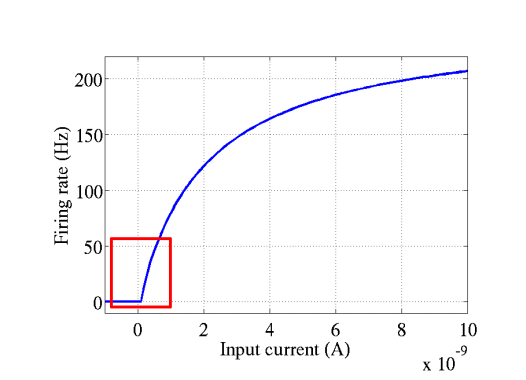
\includegraphics[width=0.5\textwidth]{imgs/firing_rate.png}
        \caption{Fréquence d'impulsions en fonction de l'intensité d'un neurone biologique (figure tirée de \cite{pmlr-v15-glorot11a}).}
        \label{fig_firing_rate}
    \end{figure}

    \begin{figure}
        \centering
        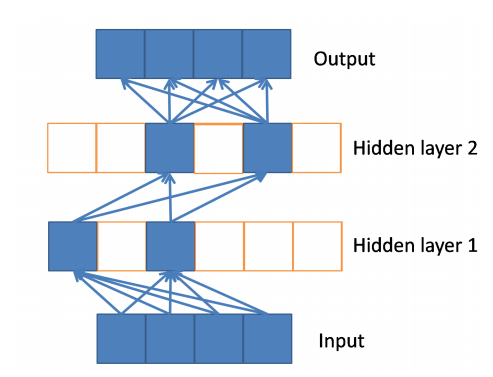
\includegraphics[width=0.5\textwidth]{imgs/sparsity.png}
        \caption{Réseau (perceptron avec deux couches cachées) utilisant la fonction d'activation RELU (figure tirée de \cite{pmlr-v15-glorot11a}). 
        Les cases blanches représentent les neurones dont le RELU renvoie 0. 
        Les cases bleues représentent les neurones dont le RELU renvoie une valeur non nulle (strictement positive).}
        \label{fig_sparsity}
    \end{figure}

    La fonction d'erreur est l'entropie croisée qui donne une mesure d'erreur pour un problème de classification.
    $E = -\frac{1}{m} \sum\limits_{i=1}^m\sum\limits_{k=1}^K (y_{k}^{(i)} \times ln(\hat{p}_{k}^{(i)}))$

    $y_{k}^{(i)}$ vaut 1 si le ième élément de l'échantillon appartient à la classe $k$, 0 sinon. $\hat{p}_{k}^{(i)}$ est la kème sortie du perceptron pour le ième élément de l'échantillon.
    
    Si le réseau a trouvé une probabilité de 1 pour la classe correspondant à l'individu alors l'erreur est nulle.
    Sinon l'erreur croit exponentiellement quand la probabilité tend vers 0. L'entropie croisée pénalise donc très fortement les grosses erreurs et faiblement les petites erreurs.
    \begin{figure}
        \centering
        \includegraphics[width=0.5\textwidth]{imgs/moins_ln.png}
        \caption{f(x)=-ln(x)}
        \label{fig_moins_ln}
    \end{figure}

    \section{Entrainement d'un réseau de neurones de classification}
    Dans cette partie l'objectif est d'entrainer notre réseau de neurones.
    L'entrainement d'un réseau de neurones consiste à régler les paramètres (poids des connexions) afin de minimiser la fonction d'erreur (l'entropie croisée dans notre cas).
    Cette minimisation est réalisée par une descente de gradient: le gradient de la fonction d'erreur est calculé puis les poids sont mis à jour et on recommence jusqu'à atteindre un minimum.
    La mise à jour est réalisée de la manière suivante:
    \begin{equation}
        \nonumber
        W := W - \eta \frac{\partial E}{\partial W}
    \end{equation}
    Nous avons donc besoin de calculer les dérivées partielles de l'erreur par rapport à chacun des poids.
    \subsection{Notation}

    Nous détaillons l'ensemble des notations pour notre perceptron ayant une couche cachée.

    $m$ est le nombre d'éléments dans notre ensemble d'entrainement.

    $K$ est le nombre de classes (et donc de sorties de notre réseau de neurones). K=3 dans notre cas.

    $n_{in}$ est le nombre de neurones de la couche d'entrée (sans le biais). 
    Donc $n_{in}$ correspond à la dimension de nos données d'entrée. $n_{in} = 13$ dans notre cas.

    $n_{hidden}$ est le nombre de neurones de la couche cachée (sans le biais). $n_{hidden}$ est un hyperparamètre (donc réglable avant l'entrainement).

    $b_i^{(l)}$ est le biais de la couche $l$ allant vers le ième neurone de la couche $l+1$.

    $w_{ij}^{(l)}$ est le poids entre le neurone $i$ de la couche $l$ et le neurone $j$ de la couche $l+1$.
    
    $(x^{(p,l)})_{i}$ est la sortie du neurone $i$ de la couche $l$ pour le $p^{eme}$ individu d'entrainement. 
    Donc $(x^{(p,2)})_{i} = relu(\sum\limits_{k=1}^{n_{in}} w_{ki}^{(1)}(x^{(p,1)})_{k} + b_i^{(1)})$
    
    $relu(x) = max(0,x)$ est la fonction d'activation de la couche cachée.

    $softmax(x)_j = \frac{e^{x_j}}{\sum\limits_{k=1}^K e^{x_k}}$ est la fonction de sortie permettant d'obtenir la probabilité pour chaque classe.

    \subsection{Calcul des dérivées partielles de la fonction de coût}

    L'apprentissage d'un réseau de neurones est executé à l'aide d'une descente de gradient sur la fonction de coût. Les paramètres de notre réseau sont les poids $w_{ij}^{(l)}$ et les biais $b_j^{(l)}$.
    Nous cherchons donc à calculer les dérivées partielles de la fonction de coût par rapport à ces différents paramètres. Nous commençons par montrer comment calculer $\frac{\partial E}{\partial w_{ij}^{(2)}}$ $\forall (i,j) \in \{1, ..., n_{hidden}\} \times \{1, ..., K\}.$

    Pour un lot de données entré dans le réseau nous avons les équations suivantes en partant de l'erreur:
    
    \begin{equation}
        \nonumber
        E = -\frac{1}{m} \sum\limits_{p=1}^m\sum\limits_{k=1}^K (y_{k}^{(p)} \times ln(\hat{p}_{k}^{(p)}))
    \end{equation}
avec 
    \begin{equation}
        \nonumber
        \hat{p}_{k}^{(p)} = softmax(x^{(p,3)})_k
    \end{equation}
    où $x^{(p,3)}$ est la sortie de la dernière couche avant le softmax pour la pème donnée d'entrainement.

    \begin{equation}
        \nonumber
        \forall (i,j) \in \{1, ..., n_{hidden}\} \times \{1, ..., K\} \quad
        \frac{\partial E}{\partial w_{ij}^{(2)}} = -\frac{1}{m} \sum\limits_{p=1}^{m} \sum\limits_{k=1}^{K} y_k^{(p)} \frac{\partial ln(\hat{p}_{k}^{(p)})}{\partial w_{ij}^{(2)}}
    \end{equation}

    Règle de la chaine:
    si $y = f(u)$ et $u=g(x)=(g_1(x), ..., g_m(x))$ alors $\frac{\partial y}{\partial x_i} = \sum\limits_{l=1}^{m} \frac{\partial y}{\partial u_l} \frac{\partial u_l}{\partial x_i}$
    
    Donc en appliquant la règle de la chaine:
    
    \begin{equation}
        \nonumber
        \frac{\partial ln(\hat{p}_{k}^{(p)})}{\partial w_{ij}^{(2)}} = \frac{\partial ln(\hat{p}_{k}^{(p)})}{\partial (x^{(p,3)})_{j}} \frac{\partial (x^{(p,3)})_{j}}{\partial w_{ij}^{(2)}}
    \end{equation}

    \begin{equation}
        \nonumber
        ln(\hat{p}_{k}^{(p)})  = (x^{(p,3)})_k - ln(\sum\limits_{q=1}^{K} e^{(x^{(p,3)})_q})
    \end{equation}

    Si $k \ne j$
    \begin{equation}
        \nonumber
        \frac{\partial ln(\hat{p}_{k}^{(p)})}{\partial (x^{(p,3)})_{j}} = -\frac{e^{(x^{(p,3)})_j}}{\sum\limits_{q=1}^{K} e^{(x^{(p,3)})_q}} = -softmax(x^{(p,3)})_j
    \end{equation}

    Sinon (dans le cas où $k = j$):
    \begin{equation}
        \nonumber
        \frac{\partial ln(\hat{p}_{k}^{(p)})}{\partial (x^{(p,3)})_{j}} = 1 - softmax(x^{(p,3)})_j
    \end{equation}

    Donc $\forall k$:
    \begin{equation}
        \frac{\partial ln(\hat{p}_{k}^{(p)})}{\partial (x^{(p,3)})_{j}} = \delta_{kj} - softmax(x^{(p,3)})_j
        \label{log_x3}
    \end{equation}
    
    où $ \delta_{kj} = 1$ si $k = j$, $0$ sinon.
    
    De plus,
    \begin{equation}
        \nonumber
        (x^{(p,3)})_{j} = \sum\limits_{i=1}^{n_{hidden}} w_{ij}^{(2)}(x^{(p,2)})_i + b_j^{(2)}
    \end{equation}

    Donc,
    \begin{equation}
        \nonumber
        \frac{\partial (x^{(p,3)})_{q}}{\partial w^{(2)}_{ij}} = (x^{(p,2)})_i
    \end{equation}

    \begin{equation}
        \nonumber
        \frac{\partial ln(\hat{p}_{k}^{(p)})}{\partial w^{(2)}_{ij}} = \bigg[ \delta_{kj} - softmax(x^{(p,3)})_j \bigg] (x^{(p,2)})_{i}
    \end{equation}

    Ce qui donne finalement:
    \begin{equation}
        \nonumber
        \frac{\partial E}{\partial w_{ij}^{(2)}} = -\frac{1}{m} \sum\limits_{p=1}^{m} \sum\limits_{k=1}^{K} y_k^{(p)} \bigg[ \delta_{kj} - softmax(x^{(p,3)})_j \bigg] (x^{(p,2)})_{i}
    \end{equation}

    Cette formule peut être interprétée de la manière suivante:
    \begin{itemize}
        \item Si la classe à prédire pour la $p^{eme}$ donnée entrée dans le réseau est $j$ alors le poids $w_{ij}^{(2)}$ est modifié en fonction de la performance de la prédiction et de $(x^{(p,2)})_{i}$.
        Si la prédiction est déjà très bonne, $w_{ij}^{(2)}$ n'est est que légèrement modifié sinon il est fortement modifié pour augmenter la probabilité sortante du réseau.
        \item Si la classe à prédire est $k \ne j$ alors il y une diminution du poids en fonction de la probabilité sortante et de $(x^{(p,2)})_{i}$. Si la probabilité sortante est faible, le poids n'est que légèrement modifié. Si elle est élevée (alors qu'elle devrait être faible), le poids est fortement modifié.
    \end{itemize}

    Nous appliquons le même procédé pour calculer $\frac{\partial E}{\partial w_{ij}^{(1)}}$

    \begin{equation}
        \frac{\partial E}{\partial w_{ij}^{(1)}} = -\frac{1}{m} \sum\limits_{p=1}^{m} \sum\limits_{k=1}^{K} y_k^{(p)} \frac{\partial ln(\hat{p}_{k}^{(p)})}{\partial w_{ij}^{(1)}}
        \label{E_wij1}
    \end{equation}

    \begin{equation}
        \frac{\partial ln(\hat{p}_{k}^{(p)})}{\partial w_{ij}^{(1)}} = \frac{\partial ln(\hat{p}_{k}^{(p)})}{\partial (x^{(p,2)})_j} \frac{\partial (x^{(p,2)})_j}{\partial w_{ij}^{(1)}}
        \label{log_wij}
    \end{equation}

    \begin{equation}
        \frac{\partial ln(\hat{p}_{k}^{(p)})}{\partial (x^{(p,2)})_j} = \sum\limits_{q=1}^{K} \frac{\partial ln(\hat{p}_{k}^{(p)})}{\partial (x^{(p,3)})_q} \frac{\partial (x^{(p,3)})_q}{\partial (x^{(p,2)})_j}
        \label{log_x2}
    \end{equation}
    
    \begin{equation}
        \frac{\partial (x^{(p,3)})_k}{\partial (x^{(p,2)})_j} = w_{jk}^{(2)}
        \label{x3_x2}
    \end{equation}
    
    D'après les équations \eqref{log_x3}, \eqref{log_x2}, \eqref{x3_x2}:
    \begin{equation}
        \frac{\partial ln(\hat{p}_{k}^{(p)})}{\partial (x^{(p,2)})_j} = \sum\limits_{q=1}^{K} \bigg[ \delta_{kq} - softmax(x^{(p,3)})_q \bigg] w_{jk}^{(2)}
        \label{log_x2_final}
    \end{equation}
    
    \begin{equation}
        \nonumber
        (x^{(p,2)})_{j} = relu\bigg[\sum\limits_{k=1}^{n_{in}} w_{kj}^{(1)}(x^{(p,1)})_{k} + b_j^{(1)}\bigg]
    \end{equation}
    
    Si $\sum\limits_{k=1}^{n_{in}} w_{kj}^{(1)}(x^{(p,1)})_{k} + b_j^{(1)} > 0$:
    \begin{equation}
        \nonumber
        \frac{\partial (x^{(p,2)})_j}{\partial w_{ij}^{(1)}} = \frac{\partial relu\bigg[\sum\limits_{k=1}^{n_{in}} w_{kj}^{(1)}(x^{(p,1)})_{k} + b_j^{(1)}\bigg]}{\partial w_{ij}^{(1)}} = \frac{\partial \bigg[\sum\limits_{k=1}^{n_{in}} w_{kj}^{(1)}(x^{(p,1)})_{k} + b_j^{(1)}\bigg]}{\partial w_{ij}^{(1)}} = (x^{(p,1)})_i
    \end{equation}
    
    Si $\sum\limits_{k=1}^{n_{in}} w_{kj}^{(1)}(x^{(p,1)})_{k} + b_j^{(1)} < 0$:
    \begin{equation}
        \nonumber
        \frac{\partial (x^{(p,2)})_j}{\partial w_{ij}^{(1)}} = \frac{\partial relu\bigg[\sum\limits_{k=1}^{n_{in}} w_{kj}^{(1)}(x^{(p,1)})_{k} + b_j^{(1)}\bigg]}{\partial w_{ij}^{(1)}} = 0
    \end{equation}
    
    Donc:
    \begin{equation}
        \frac{\partial (x^{(p,2)})_j}{\partial w_{ij}^{(1)}} = H\bigg[\sum\limits_{k=1}^{n_{in}} w_{kj}^{(1)}(x^{(p,1)})_{k} + b_j^{(1)}\bigg](x^{(p,1)})_i
        \label{x2_wij}
    \end{equation}
    où $H(x) = 1$ si $x>0$, et $0$ si $x<0$.

    %16,19,23
    D'après les équations \eqref{log_wij}, \eqref{log_x2_final}, \eqref{x2_wij}:
    \begin{equation}
        \frac{\partial ln(\hat{p}_{k}^{(p)})}{\partial w_{ij}^{(1)}} = H\bigg[\sum\limits_{q=1}^{n_{in}} w_{qj}^{(1)}(x^{(p,1)})_{q} + b_j^{(1)}\bigg](x^{(p,1)})_i \sum\limits_{q=1}^{K} \bigg[\big[ \delta_{kq} - softmax(x^{(p,3)})_q \big] w_{jq}^{(2)} \bigg] 
        \label{log_wij_final}
    \end{equation}

    D'après les équations \eqref{E_wij1} et \eqref{log_wij_final}:
    \begin{equation}
        \nonumber
        \frac{\partial E}{\partial w_{ij}^{(1)}} = -\frac{1}{m}  \sum\limits_{k=1}^{K} \sum\limits_{p=1}^{m} \Bigg[ y_k^{(p)} \sum\limits_{q=1}^{K} \bigg[ \big[ \delta_{kq} - softmax(x^{(p,3)})_q \big] w_{jq}^{(2)} \bigg] H\big[\sum\limits_{q=1}^{n_{in}} w_{qj}^{(1)}(x^{(p,1)})_{q} + b_j^{(1)}\big](x^{(p,1)})_i \Bigg]
    \end{equation}

    % Autre écriture:

    % \begin{equation}
    %     \frac{\partial E}{\partial w_{ij}^{(1)}} = -\frac{1}{m} \sum\limits_{p=1}^{m} \Bigg[ H\big[\sum\limits_{q=1}^{n_{in}} w_{qj}^{(1)}(x^{(p,1)})_{q} + b_j^{(1)}\big](x^{(p,1)})_i   \sum\limits_{k=1}^{K} \bigg[ y_k^{(p)} \sum\limits_{q=1}^{K} \Big[ \big[ \delta_{kq} - softmax(x^{(p,3)})_q \big] w_{jq}^{(2)} \Big] \bigg] \Bigg]
    % \end{equation}

    Interprétation:
    d'après la formule précédente, le changement de $w_{ij}^{(1)}$ est déterminé de la façon suivante:
    \begin{itemize}
        \item nous réunissons tous les éléments d'entrainement par classe (interprétation de la double somme et de $y_k^{(p)}$)
        \item pour chaque élément de la classe nous calculons la responsabilité de $w_{ij}^{(1)}$ dans l'erreur finale: si pour l'élément choisi, la somme pondérée est négative alors le poids n'est pas modifié (pas de responsabilité dans l'erreur, représenté par H dans l'équation)
        \item sinon la modification est proportionnelle à $(x^{(p,1)})_i$ (la variable d'entrée pour le $p^{eme}$ élément d'entrainement) 
        \item la modification est aussi proportionnelle aux erreurs de toutes les sorties (les couches sont totalement connectées ce qui est visible dans $\sum\limits_{q=1}^{K} \bigg[ \big[ \delta_{kq} - softmax(x^{(p,3)})_q \big] w_{jq}^{(2)} \bigg]$)
    \end{itemize}
    % \begin{equation}
    %     x^{(3)} = (x^{(3)}_1, ..., x^{(3)}_{K}) = (\sum\limits_{k=1}^{n_{hidden}} w_{k1}^{(2)}x_{k}^{(2)} + b_1^{(2)}, ..., \sum\limits_{k=1}^{n_{hidden}} w_{kK}^{(2)}x_{k}^{(2)} + b_{K}^{(2)})
    % \end{equation}

    \section{Rétropropagation}
    \subsection{Calcul des gradients à l'aide de la rétropropagation}
    Nous avons montré dans la section précédente comment calculer les dérivées partielles de la fonction de coût. Cependant les calculs deviennent rapidement assez complexes et peu efficaces en terme de performances.
    Il va être très compliqué d'ajouter des couches cachées supplémentaires à notre réseau.
    Nous allons détailler l'algorithme de rétropropagation du gradient qui permet de calculer les gradients successivements en appliquant astucieusement la règle de la chaîne.
    L'algorithme de rétropropagation consiste à calculer $\frac{\partial E}{\partial w_{ij}^{(1)}}$ en réutilisant une partie des calculs faits pour $\frac{\partial E}{\partial w_{ij}^{(2)}}$.

    Soit $E^p$ l'erreur pour la $p^{eme}$ donnée:
    \begin{equation}
        \nonumber
        E^p = - \sum\limits_{k=1}^K (y_{k}^{(p)} \times ln(\hat{p}_{k}^{(p)}))
    \end{equation}

    En appliquant la règle de la chaine:
    \begin{equation}
        \begin{aligned}
            \nonumber
            \frac{\partial E^p}{\partial w_{ij}^{(1)}} & = \frac{\partial E^p}{\partial (x^{(p,2)})_j} \frac{\partial (x^{(p,2)})_j}{\partial (\sum\limits_{k=1}^{n_{in}} w_{kj}^{(1)}(x^{(p,1)})_{k} + b_j^{(1)})} \frac{\partial (\sum\limits_{k=1}^{n_{in}} w_{kj}^{(1)}(x^{(p,1)})_{k} + b_j^{(1)})}{\partial w_{ij}^{(1)}} \\
            & = \frac{\partial E^p}{\partial (x^{(p,2)})_j} H\big[\sum\limits_{q=1}^{n_{in}} w_{qj}^{(1)}(x^{(p,1)})_{q} + b_j^{(1)}\big] (x^{(p,1)})_i
        \end{aligned}
    \end{equation}

    Il reste à calculer $\frac{\partial E^p}{\partial (x^{(p,2)})_j}$:
    \begin{equation}
        \nonumber
        \frac{\partial E^p}{\partial (x^{(p,2)})_j}  = \sum\limits_{k=1}^{K} \Big(\frac{\partial E^p}{\partial (x^{(p,3)})_k} \frac{\partial (x^{(p,3)})_k}{\partial (x^{(p,2)})_j}\Big) = \sum\limits_{k=1}^{K} \Big(\frac{\partial E^p}{\partial (x^{(p,3)})_k} w_{jk}^{(2)}\Big)
    \end{equation}

    D'après les deux équations précédentes:

    \begin{equation}
        \nonumber
        \frac{\partial E^p}{\partial w_{ij}^{(1)}} = \sum\limits_{k=1}^{K} \Big(\frac{\partial E^p}{\partial (x^{(p,3)})_k} w_{jk}^{(2)}\Big) H\big[\sum\limits_{q=1}^{n_{in}} w_{qj}^{(1)}(x^{(p,1)})_{q} + b_j^{(1)}\big] (x^{(p,1)})_i
    \end{equation}

    Donc

    \begin{equation}
        \frac{\partial E}{\partial w_{ij}^{(1)}} = \frac{1}{m}\sum\limits_{p=1}^{m}\sum\limits_{k=1}^{K} \Big(\frac{\partial E^p}{\partial (x^{(p,3)})_k} w_{jk}^{(2)}\Big) H\big[\sum\limits_{q=1}^{n_{in}} w_{qj}^{(1)}(x^{(p,1)})_{q} + b_j^{(1)}\big] (x^{(p,1)})_i
        \label{backprop}
    \end{equation}

    Si $\frac{\partial E}{\partial w_{ij}^{(2)}}$ a déjà été calculé alors $\frac{\partial E}{\partial w_{ij}^{(1)}}$ est calculable. En effet, les $\frac{\partial E^p}{\partial (x^{(p,3)})_k}$ sont calculés pour $\frac{\partial E}{\partial w_{ij}^{(2)}}$.
    Les gradients d'une couche $l$ sont sonc calculés en fonction de ce qui a déjà été calculé pour la couche $l+1$.

    \subsection{Algorithme d'apprentissage d'un réseau de neurones}

    L'apprentissage du réseau de neurones consiste à calculer les gradients de la fonction erreur par rapport aux poids du réseau à l'aide des équations suivantes (rétropropagation) puis à faire une descente de gradients.
    Les poids sont initialisés avec une loi normale d'espérance 0 et de variance 1.

    \begin{equation}
        \nonumber
        \frac{\partial E^p}{\partial (x^{(p,3)})_{j}} = -\sum\limits_{k=1}^{K} y_k^{(p)} \frac{\partial ln(\hat{p}_{k}^{(p)})}{\partial (x^{(p,3)})_{j}} = - \sum\limits_{k=1}^{K} y_k^{(p)} \bigg[ \delta_{kj} - softmax(x^{(p,3)})_j \bigg]
    \end{equation}

    \begin{equation}
        \nonumber
        \frac{\partial E^p}{\partial w_{ij}^{(2)}} = \frac{\partial E^p}{\partial (x^{(p,3)})_{j}} \frac{\partial (x^{(p,3)})_{j}}{\partial w_{ij}^{(2)}} = \frac{\partial E^p}{\partial (x^{(p,3)})_{j}} (x^{(p,2)})_i
    \end{equation}

    \begin{equation}
        \nonumber
        \frac{\partial E}{\partial w_{ij}^{(2)}} = \frac{1}{m} \sum\limits_{p=1}^{m} \frac{\partial E^p}{\partial w_{ij}^{(2)}}
    \end{equation}

    \begin{equation}
        \nonumber
        \frac{\partial E^p}{\partial b_j^{(2)}} = \frac{\partial E^p}{\partial (x^{(p,3)})_{j}} \frac{\partial (x^{(p,3)})_{j}}{\partial b_{j}^{(2)}} = \frac{\partial E^p}{\partial (x^{(p,3)})_{j}}
    \end{equation}

    \begin{equation}
        \nonumber
        \frac{\partial E}{\partial b_{j}^{(2)}} = \frac{1}{m} \sum\limits_{p=1}^{m} \frac{\partial E^p}{\partial b_{j}^{(2)}}
    \end{equation}

    \begin{equation}
        \nonumber
        \frac{\partial E^p}{\partial w_{ij}^{(1)}} = \sum\limits_{k=1}^{K} \Big(\frac{\partial E^p}{\partial (x^{(p,3)})_k} w_{jk}^{(2)}\Big) H\big[\sum\limits_{q=1}^{n_{in}} w_{qj}^{(1)}(x^{(p,1)})_{q} + b_j^{(1)}\big] (x^{(p,1)})_i
    \end{equation}

    \begin{equation}
        \nonumber
        \frac{\partial E}{\partial w_{ij}^{(1)}} = \frac{1}{m}\sum\limits_{p=1}^{m}\frac{\partial E^p}{\partial w_{ij}^{(1)}}
    \end{equation}

    \begin{equation}
        \nonumber
        \frac{\partial E^p}{\partial b_j^{(1)}} = \sum\limits_{k=1}^{K} \Big(\frac{\partial E^p}{\partial (x^{(p,3)})_k} w_{jk}^{(2)}\Big) H\big[\sum\limits_{q=1}^{n_{in}} w_{qj}^{(1)}(x^{(p,1)})_{q} + b_j^{(1)}\big]
    \end{equation}

    \begin{equation}
        \nonumber
        \frac{\partial E}{\partial b_j^{(1)}} = \frac{1}{m}\sum\limits_{p=1}^{m}\frac{\partial E^p}{\partial b_j^{(1)}}
    \end{equation}



    \begin{lstlisting}[mathescape]
        initialisation aleatoire de tous les poids
        faire
            pour chaque exemple d'entrainement
                prediction: calcul de $x^{(p,2)}$, $x^{(p,3)}$, et $softmax(x^{(p,3)})$
                pour chaque $j \in \{1, ..., K\}$
                    calcul de $\frac{\partial E^p}{\partial (x^{(p,3)})_{j}}$
                pour chaque $(i,j) \in \{1, ..., n_{hidden}\} \times \{1, ..., K\}$
                    calcul de $\frac{\partial E^p}{\partial w_{ij}^{(2)}}$
                pour chaque $(i,j) \in \{1, ..., n_{in}\} \times \{1, ..., n_{hidden}\}$
                    calcul de $\frac{\partial E^p}{\partial w_{ij}^{(1)}}$
                pour chaque $j \in \{1, ..., K\}$
                    calcul de $\frac{\partial E^p}{\partial b_{j}^{(2)}}$
                pour chaque $j \in \{1, ..., n_{hidden}\}$
                    calcul de $\frac{\partial E^p}{\partial b_{j}^{(1)}}$
            pour chaque $(i,j) \in \{1, ..., n_{hidden}\} \times \{1, ..., K\}$
                calcul de $\frac{\partial E}{\partial w_{ij}^{(2)}}$ (moyenne de $\frac{\partial E^p}{\partial w_{ij}^{(2)}}$)
            pour chaque $(i,j) \in \{1, ..., n_{in}\} \times \{1, ..., n_{hidden}\}$
                calcul de $\frac{\partial E}{\partial w_{ij}^{(1)}}$ (moyenne de $\frac{\partial E^p}{\partial w_{ij}^{(1)}}$)
            pour chaque $j \in \{1, ..., K\}$
                calcul de $\frac{\partial E}{\partial b_{j}^{(2)}}$
            pour chaque $j \in \{1, ..., n_{hidden}\}$
                calcul de $\frac{\partial E}{\partial b_{j}^{(1)}}$
            Mise a jour des poids: $W = W - \eta \frac{\partial E}{\partial W}$ (descente de gradients)
            Mise a jour des biais: $b = b - \eta \frac{\partial E}{\partial b}$ (descente de gradients)
        jusqu'a ce que tous les exemples d'entrainement soient tries 
        correctement (ou tout autre critere d'arret)
    \end{lstlisting}

    \section{Implémentation}
    Nous avons implémentaté ce perceptron à une couche et l'avons entrainé sur le jeu de données indiqué en première partie.
    Les 3 classes ayant à peu près le même effectif nous avons calculé le nombre d'erreurs divisé par l'effectif total sur un ensemble de test représentant 30\% des données (le reste servant à l'entrainement).
    
    \begin{tabular}{|l|l|l|}
        \hline
        Nombre de neurones dans la couche cachée & Pourcentage d'erreur \\\hline  \hline
        5 & 39\% \\ \hline
        10 & 6\% \\ \hline
        30 & 6\% \\ \hline
        50 & 2\% \\ \hline
        100 & 0\% \\ \hline
        1000 & 0\% \\ \hline
    \end{tabular}
    \bibliographystyle{plain}
    \bibliography{bibtex.bib}

    \end{document}